\section{Evaluation}
\label{sec:exec_time_prediction.evaluation}

\subsection{Experimental Setup}
\label{sec:exec_time_prediction.evaluation.setup}

% Benchmark descriptions
\begin{table*}
  \begin{center}
    \begin{footnotesize}
    \begin{tabular}{|l||l|l||r|r|r|}

\hline
\multirow{2}{*}{\bf Benchmark} & \multirow{2}{*}{\bf Description} & \multirow{2}{*}{\bf Task} & \multicolumn{3}{c|}{\bf{Job Times [ms]}} \\ \cline{4-6}
& & & {\bf Min} & {\bf Avg} & {\bf Max} \\ \hline\hline


2048 \cite{2048} & Puzzle game & Update and render one turn &
  0.52 & 1.2 & 2.1 \\ \hline
curseofwar \cite{curseofwar} & Real-time strategy game & Update and render one game loop iteration &
  0.02 & 6.2 & 37.2 \\ \hline
ldecode \cite{ldecode} & H.264 decoder & Decode one frame & 
  6.2 & 20.4 & 32.5 \\ \hline
pocketsphinx \cite{pocketsphinx-icassp06} & Speech recognition & Process one speech sample & 
  718 & 1661 & 2951 \\ \hline
rijndael \cite{mibench} & Advanced Encryption Standard (AES) & Encrypt one piece of data & 
  14.2 & 28.5 & 43.6 \\ \hline
sha \cite{mibench} & Secure Hash Algorithm (SHA) & Hash one piece of data & 
  4.7 & 25.3 & 46.0 \\ \hline
%stringsearch \cite{mibench} & Search for words in phrases & Perform a set of searches \\ \hline
uzbl \cite{uzbl} & Web browser & Execute one command (e.g., refresh page) & 
  0.04 & 2.2 & 35.5 \\ \hline
xpilot \cite{xpilot} & 2D space game & Update and render one game loop iteration & 
  0.2 & 1.3 & 3.1 \\ \hline


\end{tabular}

    \end{footnotesize}
    \caption{Benchmark descriptions and task of interest.}
    \label{tab:exec_time_prediction.evaluation.benchmarks}
  \end{center}
\end{table*}

% Benchmark execution times
\begin{table*}
  \begin{center}
    \begin{footnotesize}
    \begin{tabular}{|l|r|r|r|}

\hline
{\bf Benchmark} & {\bf Min [ms]} & {\bf Avg. [ms]} & {\bf Max [ms]} \\ \hline\hline

2048         & 0.52 &  1.2 &  2.1 \\ \hline
curseofwar   & 0.02 &  6.2 & 37.2 \\ \hline
ldecode      & 6.2  & 20.4 & 32.5 \\ \hline
pocketsphinx & 718  & 1661 & 2951 \\ \hline
rijndael     & 14.2 & 28.5 & 43.6 \\ \hline
sha          & 4.7  & 25.3 & 46.0 \\ \hline
uzbl         & 0.04 & 2.2  & 35.5 \\ \hline
xpilot       & 0.2  & 1.3  & 3.1 \\ \hline

\end{tabular}

    \end{footnotesize}
    \caption{Execution time statistics when running
    at maximum frequency.}
    \label{tab:exec_time_prediction.evaluation.job_statistics}
  \end{center}
\end{table*}

We applied our framework for prediction-based DVFS control to a set of eight
benchmark applications including three games, a web browser, speech
recognition, a video decoder and two applications from the MiBench suite
\cite{mibench}.  Table~\ref{tab:exec_time_prediction.evaluation.benchmarks}
lists and describes these benchmarks and the task of interest for each.
Table~\ref{tab:exec_time_prediction.evaluation.job_statistics} shows the
minimum, average, and maximum job execution times for these benchmarks when run
at maximum frequency.

We ran our experiments on an ODROID-XU3 \cite{odroid} development board running
Ubuntu 14.04. The ODROID-XU3 includes a Samsung Exynos5422 SoC with ARM
Cortex-A15 and Cortex-A7 cores. We show results here for running on the more
power-efficient A7 core but we saw similar trends when running on the A15 core.
In order to isolate measurements for the application of interest, we pinned the
benchmark to run on the A7 core while using the A15 to run OS and background
jobs. We measured power using the on-board power sensors with a sampling rate
of 213 samples per second and integrated over time to calculate energy usage.

We compare our proposed prediction-based DVFS controller with existing
controllers and previously proposed control schemes. Specifically, we measure
results for the following DVFS schemes:
\begin{enumerate}
  \item \textbf{performance}: The Linux performance governor
  \cite{linux_governors} always runs at the maximum frequency. We normalize our
  energy results to this case.
  \item \textbf{interactive}: The Linux interactive governor
  \cite{linux_governors} was designed for interactive mobile applications. It
  samples CPU utilization every 80 milliseconds and changes to maximum
  frequency if CPU utilization is above 85\%.
  \item \textbf{pid}: The PID-based controller uses previous prediction errors
  with a PID control algorithm in order to predict the execution time of the
  next job \cite{gu-dac08}. The PID parameters are trained offline and are
  optimized to reduce deadline misses.
  \item \textbf{prediction}: This is our prediction-based controller as
  described in this chapter.
\end{enumerate}

\subsection{Energy Savings and Deadline Misses}

% Energy, deadline misses
\begin{figure*}
  \begin{center}
    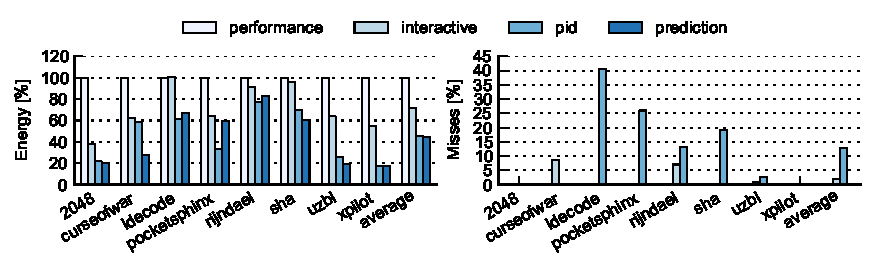
\includegraphics{exec_time_prediction/data/em_summary.pdf}
    \caption{Normalized energy usage and deadline misses.}
    \label{fig:exec_time_prediction.evaluation.em_summary}
  \end{center}
\end{figure*}

Figure~\ref{fig:exec_time_prediction.evaluation.em_summary} compares energy
consumption and deadline misses for the different DVFS controllers across our
benchmark set. These experiments are run with a time budget of 50 milliseconds per job as
running faster than this is not noticeable to a user \cite{lindgaard-bit06,
eqos-hpca15}.  pocketsphinx takes at least 100s of milliseconds to run (see
Table~\ref{tab:exec_time_prediction.evaluation.benchmarks}) so we use a 4
second deadline. This corresponds to the time limit that a user is willing to
wait for a response \cite{miller-afips68}.  Energy numbers are normalized to
the energy usage of the performance governor.  Deadline misses are reported as
the percentage of jobs that miss their deadline. 

We see that, on average, our prediction-based controller saves 56\% energy
compared to running at max frequency. This is 27\% more savings than the
interactive governor and 1\% more savings than the PID-based controller.  For
ldecode, pocketsphinx, and rijndael, prediction-based control shows higher
energy consumption than PID-based control. However, if we look at deadline
misses, we see that PID-based control shows a large number of misses for these
benchmarks. On average, the interactive governor shows 2\% deadline misses and
the PID-based controller shows 13\% misses. In contrast, our prediction-based
controller shows 0.1\% deadline misses for curseofwar and no deadline misses
for the other benchmarks tested. Overall, we see that the interactive governor
has a low number of deadline misses, but achieves this with high energy
consumption. On the other hand, PID-based control shows lower energy usage than
the prediction-based controller in some cases, but this comes at the cost of a
large number of deadline misses. Instead, on average, our prediction-based
control is able to achieve both better energy consumption and less deadline
misses than the interactive governor and PID-based control.

% Deadline sweeps
\begin{figure*}
  \begin{center}
  \begin{subfigure}[2048]{
    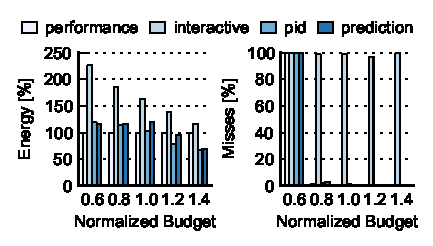
\includegraphics{exec_time_prediction/data/2048.pdf}
  }
  \end{subfigure}
  \hspace{-0.3in}
  \begin{subfigure}[curseofwar]{
    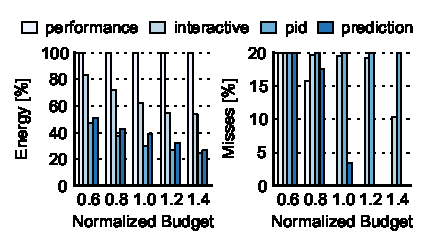
\includegraphics{exec_time_prediction/data/curseofwar.pdf}
  }
  \end{subfigure}

  \begin{subfigure}[ldecode]{
    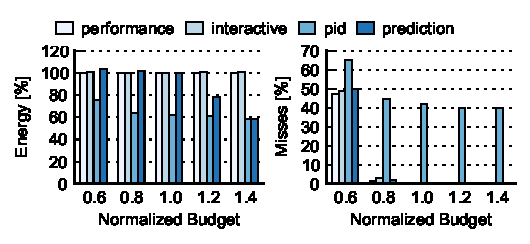
\includegraphics{exec_time_prediction/data/ldecode.pdf}
  }
  \end{subfigure}
  \hspace{-0.3in}
  \begin{subfigure}[pocketsphinx]{
    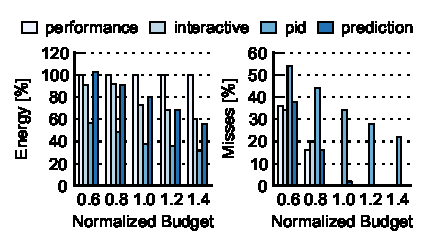
\includegraphics{exec_time_prediction/data/pocketsphinx.pdf}
  }
  \end{subfigure}

  \begin{subfigure}[rijndael]{
    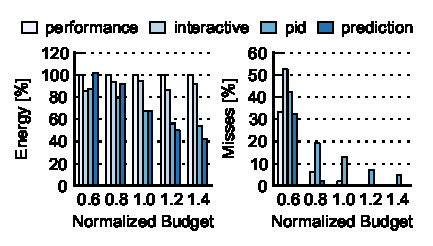
\includegraphics{exec_time_prediction/data/rijndael.pdf}
  }
  \end{subfigure}
  \hspace{-0.3in}
  \begin{subfigure}[sha]{
    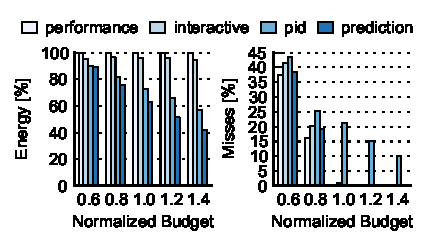
\includegraphics{exec_time_prediction/data/sha.pdf}
  }
  \end{subfigure}

  \begin{subfigure}[uzbl]{
    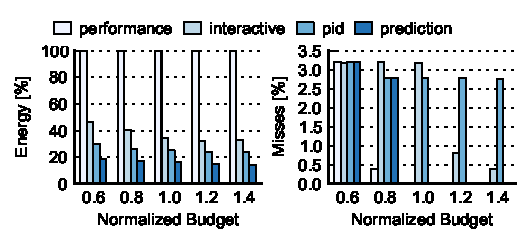
\includegraphics{exec_time_prediction/data/uzbl.pdf}
  }
  \end{subfigure}
  \hspace{-0.3in}
  \begin{subfigure}[xpilot]{
    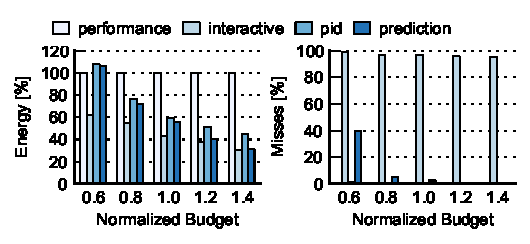
\includegraphics{exec_time_prediction/data/xpilot.pdf}
  }
  \end{subfigure}

  \caption{Normalized energy usage and deadline misses as time budget is
  varied.}
  \label{fig:exec_time_prediction.evaluation.sweeps}
  \end{center}
\end{figure*}

Since our prediction-based controller takes the time budget into account, it is
able to save more energy with longer time budgets. Similarly, with shorter time
budgets, it will spend more energy to attempt to meet the tighter deadlines.
In order to study this trade-off, we swept the time budget around the point
where we expect to start seeing deadline misses. Specifically, we set a
normalized budget of 1 to correspond to the maximum execution time seen for the
task when running at maximum frequency (see
Table~\ref{tab:exec_time_prediction.evaluation.benchmarks}). This corresponds
to the tightest budget such that all jobs are able to meet their deadline.
Figure~\ref{fig:exec_time_prediction.evaluation.sweeps} shows the energy usage
and deadline misses for the various benchmarks as the normalized budget is
swept below and above 1.  We see that our prediction-based controller is able
to save more energy with longer time budgets and continues to outperform the
interactive governor and the PID-based controller for varying time budgets.
For normalized budgets less than 1, our prediction-based controller shows
deadline misses. However, the number of misses is typically close to the number
seen with the performance governor.  This implies that the only deadline misses
are the ones that are impossible to meet at the specified time budget, even
with running at the maximum frequency.

\subsection{Analysis of Overheads and Error}
\label{sec:exec_time_prediction.evaluation.overheads}

% Overhead time
\begin{figure}
  \begin{center}
    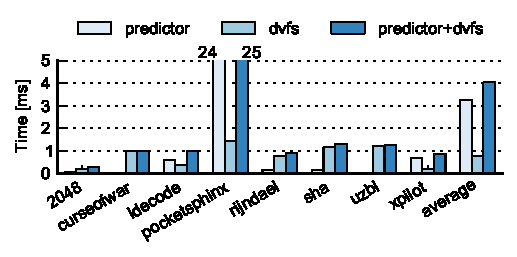
\includegraphics{exec_time_prediction/data/overhead_time.pdf}
    \caption{Average time to run prediction slice and switch DVFS levels.}
    \label{fig:exec_time_prediction.evaluation.overhead_time}
  \end{center}
\end{figure}

Figure~\ref{fig:exec_time_prediction.evaluation.overhead_time} shows the
average times for executing the predictor and for switching DVFS levels.  On
average, the predictor takes 3.2 ms to execute and DVFS switching takes 0.8 ms.
Excluding pocketsphinx, the average total overhead is less than 1 ms which is
2\% of a 50 ms time budget.  pocketsphinx shows a long execution time for the
predictor. However, this time is negligible compared to the execution time of
pocketsphinx jobs which are on the order of seconds.

% Results w/o overhead
\begin{figure}
  \begin{center}
    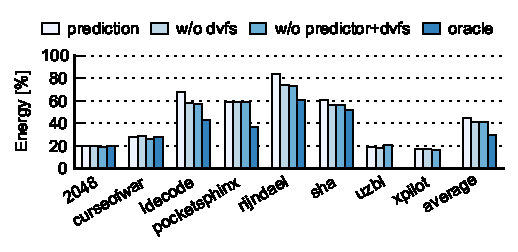
\includegraphics{exec_time_prediction/data/overhead_comparison.pdf}
    \caption{Normalized energy usage and deadline misses with overheads removed
    and oracle prediction.}
    \label{fig:exec_time_prediction.evaluation.overhead_comparison}
  \end{center}
\end{figure}

The overheads of executing the predictor and DVFS switching decrease the energy
savings achievable. This is due to the energy consumed to perform these
operations as well as the decrease in effective budget.  Better program slicing
and/or feature selection could reduce the predictor execution time.  Similarly,
faster DVFS switching circuits \cite{booster-hpca12, shortstop-vlsic13,
fgsync-micro14} have shown switching times on the order of tens of nanoseconds.
In order to explore the limits of what is achievable, we evaluated our
prediction-based control when the overheads of the predictor and DVFS switching
are ignored.
Figure~\ref{fig:exec_time_prediction.evaluation.overhead_comparison} shows the
energy and deadline misses when these overheads are removed. These results are
shown for a time budget of 4 seconds for pocketsphinx and 50 milliseconds for all other
benchmarks.  On average, we see a 3\% decrease in energy consumption when
removing the overheads of DVFS switching. Removing the overhead of running the
predictor shows negligible improvement past removing the DVFS switching
overhead.

% Prediction error
\begin{figure}
  \begin{center}
    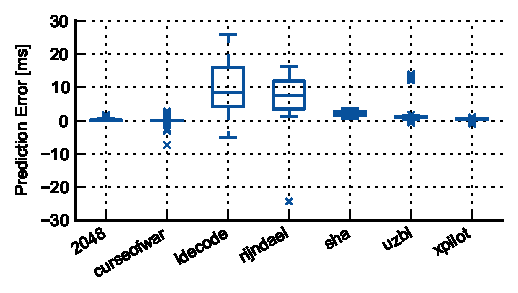
\includegraphics{exec_time_prediction/data/prediction_error.pdf}
    \caption{Box-and-whisker plots of prediction error. Positive number
    correspond to over-prediction and negative numbers correspond to
    under-prediction.}
    \label{fig:exec_time_prediction.evaluation.prediction_error}
  \end{center}
\end{figure}

In addition to these overheads, the accuracy of our prediction limits the
effectiveness of the prediction-based controller.
Figure~\ref{fig:exec_time_prediction.evaluation.prediction_error} shows
box-and-whisker plots of the prediction error.  The box indicates the first and
third quartiles and the line in the box marks the median value. Outliers
(values over 1.5 times the inner quartile range past the closest box end) are
marked with an ``x'' and the non-outlier range is marked by the whiskers.
Positive values represent over-prediction and negative-numbers represent
under-prediction. We can see that the prediction skews toward over-prediction
with average errors greater than 0.  Most benchmarks show prediction errors of
less than 5 ms, which is only 10\% of a 50 ms time budget. ldecode and rijndael
show higher prediction errors, which limits the energy savings possible.
pocketsphinx (not shown) has errors ranging from 60 ms under-prediction to 2
seconds over-prediction with an average of 880 ms over-prediction. Although
these errors are larger in absolute terms than the other benchmarks, they are
on the same order of magnitude when when compared to the execution time of
pocketsphinx jobs.

In order to explore the possible improvements with perfect prediction, we
implemented an ``oracle'' controller that uses recorded job times from a
previous run with the same inputs to predict the execution time of jobs.
Figure~\ref{fig:exec_time_prediction.evaluation.overhead_comparison} also
includes these oracle results. We see than an additional 11\% energy savings
are achievable with oracle on top of removing the predictor and DVFS switching
overheads. Note that we do not have oracle results for uzbl and xpilot as
non-deterministic variations in the ordering of jobs across runs made it
difficult to implement a good oracle controller.

\subsection{Under-prediction Trade-off}

% Under-predict trade-off
\begin{figure}
  \begin{center}
    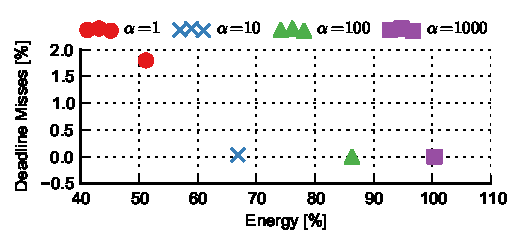
\includegraphics{exec_time_prediction/data/underpredict_sweep.pdf}
    \caption{Energy vs. deadline misses for various under-predict penalty
    weights ($\alpha$) for ldecode.}
    \label{fig:exec_time_prediction.evaluation.underpredict_sweep}
  \end{center}
\end{figure}

In Section~\ref{sec:exec_time_prediction.prediction.model}, we discussed how we
can vary the penalty weight for under-prediction, $\alpha$, when we fit our
execution time prediction model. Placing greater penalty on under-prediction
increases the energy usage but reduces the likelihood of deadline misses.
Figure~\ref{fig:exec_time_prediction.evaluation.underpredict_sweep} shows the
energy and deadline misses for varying under-predict penalty weights for
ldecode. We see that as the weight is decreased, energy consumption decreases
but deadline misses increase. Reducing the weight from 1000 to 100 keep misses
at 0, but reducing the weight to 10 introduces a small number of deadline
misses (0.03\%). Other benchmarks show similar trends and we found that across
the benchmarks we tested, an under-predict penalty weight of 100 provided good
energy savings without sacrificing deadline misses. The results in this chapter
have been shown with a weight of 100.

\subsection{Heterogeneous Cores}

% Motivation for heterogeneous cores
Recent architectures have introduced the use of heterogeneous CPU cores in
order to better match application needs. For example, ARM's big.LITTLE
architecture couples a set of large, fast cores (e.g., Cortex-A15) with a set
of small, energy-efficient cores (e.g., Cortex-A7). The big cores can be used
for tasks which need high performance while the little cores can be used to
save energy on performance-insensitive tasks. These additional operating points
can be taken advantage of with our prediction-based to provide a wider range of
operating points, providing greater energy savings at slower operating points
and/or less deadline misses using faster operating points. In this section, we
explore the possible effects of such an architecture using first-order
analytical models.

% Modification of prediction algorithm
The majority of our prediction-based methodology can be applied, unchanged, to
scheduling resources with heterogeneous cores. In addition to selecting an
appropriate frequency, the algorithm must select whether to run on the little
or big core. The first two steps of our methodology, generating program
features and predicting execution time (see
Figure~\ref{fig:exec_time_prediction.prediction.prediction_flow}, remain
unchanged. We modify the last step, predicting frequency, to predict both core
type and frequency. This is done by extending our simple linear model of
frequency-based performance scaling of a single core to be a pair of linear
models. The big core is modeled as a constant factor faster than the little
core. Based on our benchmarking on the ODROID-XU3, the big core is, on average,
2x faster than the little core.

% Evaluation setup
In order to evaluate the effects of heterogeneous cores and DVFS scaling, we
collected traces of jobs and execution times while running at maximum frequency
on the big and little cores of the ODROID-XU3. For our models, we assume that
execution time scales linearly with frequency and that energy scales
quadratically with frequency. Switching time between cores can be as low as
20,000 cycles \cite{cho-12} which corresponds to only 20 microseconds at 1 GHz.
As this switching time is small compared to our deadlines, we ignore the
switching time overhead. Note that this cited switching time only accounts for
the dead time when instructions cannot be run and does not account for cold
cache misses on the new core and syscall overheads to initiate the core
migration. However, we note that including switching overheads of several
milliseconds in our modeling results did not qualitatively change the results.
We model the power usage of the big core as approximately 3x larger than the
little core running at the same frequency using microbenchmarking results.

% Little-only vs. Big-little
\begin{figure*}
  \begin{center}
  \begin{subfigure}[Energy]{
    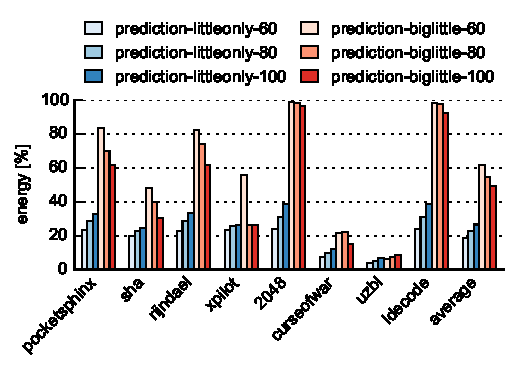
\includegraphics{exec_time_prediction/data/hetero_little_energy.pdf}
    \label{fig:exec_time_prediction.evaluation.littleonly_energy}
  }
  \end{subfigure}
  \begin{subfigure}[Deadline Misses]{
    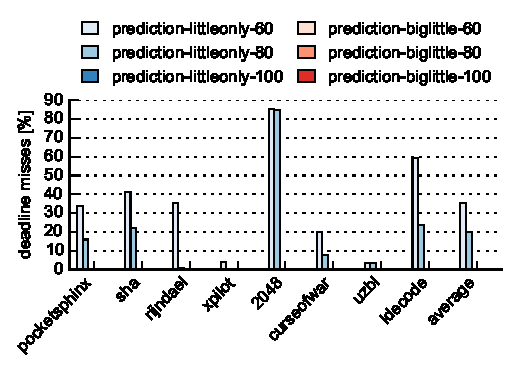
\includegraphics{exec_time_prediction/data/hetero_little_deadline_misses.pdf}
    \label{fig:exec_time_prediction.evaluation.littleonly_deadline_misses}
  }
  \end{subfigure}
  \begin{subfigure}[Switch Count]{
    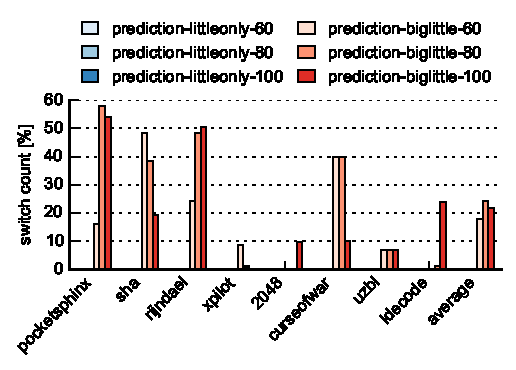
\includegraphics{exec_time_prediction/data/hetero_little_switch_count.pdf}
    \label{fig:exec_time_prediction.evaluation.littleonly_switch_count}
  }
  \end{subfigure}

  \caption{Little-only versus Big-Little}
  \label{fig:exec_time_prediction.evaluation.littleonly}
  \end{center}
\end{figure*}

% Results littleonly
We first compare the case of running only on a little core versus having a big
and little core. We set the budget based on the worst-case execution time
while running at maximum frequency. We show results for time budgets 0.6x,
0.8x, and 1.0x of the worst-case execution time.
Figure~\ref{fig:exec_time_prediction.evaluation.littleonly_energy} shows the
energy usage normalized to running at a constant frequency. This constant
frequency is the minimum needed to meet all deadlines.
Figure~\ref{fig:exec_time_prediction.evaluation.littleonly_deadline_misses}
shows the deadline misses and
Figure~\ref{fig:exec_time_prediction.evaluation.littleonly_switch_count} shows
the percentage of jobs which switch cores (i.e., from big to little or vice
versa). We see that for budgets tighter than 1.0x, deadline misses begin to
occur when only using the little core. However, by introducing the big core, we
are able to run at faster operating points and eliminate these deadline misses.
This does come at increased energy usage.

% Little-only vs. Big-little
\begin{figure*}
  \begin{center}
  \begin{subfigure}[Energy]{
    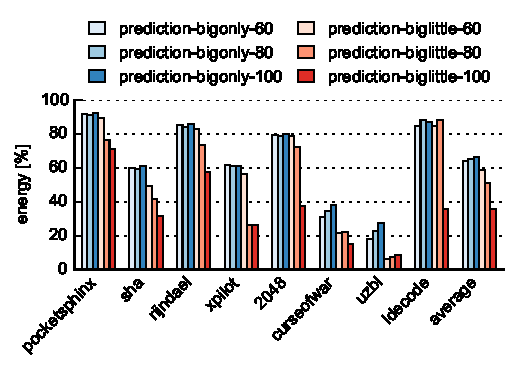
\includegraphics{exec_time_prediction/data/hetero_big_energy.pdf}
  }
  \end{subfigure}
  \begin{subfigure}[Deadline Misses]{
    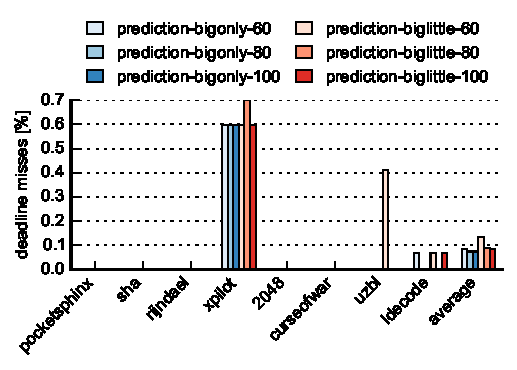
\includegraphics{exec_time_prediction/data/hetero_big_deadline_misses.pdf}
  }
  \end{subfigure}
  \begin{subfigure}[Switch Count]{
    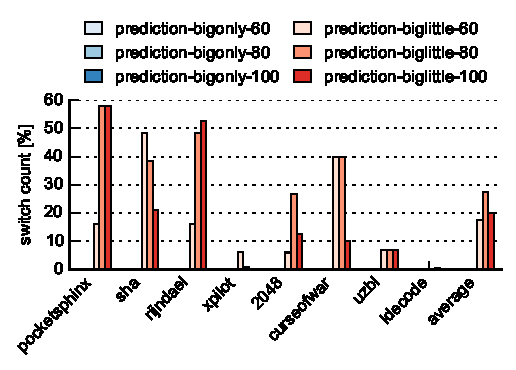
\includegraphics{exec_time_prediction/data/hetero_big_switch_count.pdf}
  }
  \end{subfigure}

  \caption{Big-only versus Big-Little}
  \label{fig:exec_time_prediction.evaluation.bigonly}
  \end{center}
\end{figure*}

% Results bigonly
We also compare the case of running only on a big core versus having big and
little cores. Figure~\ref{fig:exec_time_prediction.evaluation.bigonly} shows
the results for this setup. We see that almost no deadline misses occur in any
case, because the faster big core is able to meet all deadlines. However, lower
energy can be achieved by introducing the little core, allowing lower energy
operating points than the big core running at minimum frequency.

% Conclusions
These results show that improved energy savings and/or reduced deadline misses
can be achieved by taking advantage of heterogeneous cores. In addition, our
prediction-based methodology can be easily extended to select operating points
on such a system.
